\documentclass[journal, a4paper]{IEEEtran}


\usepackage{graphicx} 
\usepackage{url}      
\usepackage{amsmath}  \begin{document}
	\title{Robust Principal Component Analysis}
	\author{EMMANUEL J. CANDES and XIAODONG LI, Stanford University 
		\\JOHN WRIGHT, Microsoft Research Asia \\
		YI MA, University of Illinois at Urbana-Champaign,\\ Microsoft Research Asia\\
		\vspace{1cm}
		Report by: Neel Puniwala - 1401024}
		
	\maketitle
\begin{abstract}
	Basically given paper rotate around the technique that is use to recover the corrupted data of the given matrix. Data matrix is the mixture of the low rank matrix and sparse matrix. In paper, they introduce a new technique named principle component pursuit. Also the result of the paper claim that one can recover the principal component of the data matrix even though the positive fraction of its entries are arbitrarily corrupted. This concept can be extending in the situation where the entries are missing. They also discuss the applications in area of video surveillance, face recognition.\\
	Index Terms \textendash Principal Component, norm, duality, low-rank matrices, Sparsity, Video surveillance. (key words)
\end{abstract}


\section{Introduction}
	\PARstart{A}{ssume} Data matrix is M and it can decompose in low rank matrix and sparse matrix.\\
	$$M=L_0 + S_0$$\\
	Where,\\
	 $L_0$ is low rank matrix component\\
	 $S_0$ is Sparse matrix component\\
	\\Where we do not know the dimension of the Low rank matrix and not even their low-dimensional column and row space. And we also do not know about place of nonzero entries of Sparse matrix. Now a day’s massive amount of high dimensional data is challenged for the science. Such type of data has low dimensionality can be lie in some low dimensional sub-space. 
	
	$$M = L_0 + N_0 $$\\
	Where $L_0$ is low rank matrix and $N_0$ is small perturbation matrix. Rank of the $L_0$ is k can be solving by
$$Minimize  || M \textendash L ||$$
$$ Subject to rank(L) \leq k$$

Where $|| M ||$ denotes the 2-norm of matrix M. When $N_0$ is small and independent and identically distributed then it could be solved using singular value decomposition.  But when the data matrix is highly corrupted we cannot recover the data matrix using classical SVD for that concept of Robust principal component analysis is helpful. It is a modification of PCA. It is mainly used to reduce the dimension of the data matrix. Decomposition can be done using techniques called Principal component pursuit(PCA). They discuss one very good real life application Ranking and collaborative filtering. In this application they mentioned that to improve the user browsing experience most of the company collect user searching data which is incomplete most of the time. So we estimate some data and based on that we fit data into sparse and low rank matrix. 

% Main Part
\section{IMPORTANT CONCEPT}
	Before, get into the technique which suggested in paper we need to understand certain concept like different type of norms which are used in PCP (Principle component pursuit). Basically, Norm is a total size or length of vectors in vector space. Norm can be shown using $|| x ||$. If vector v= [1 2 4] 
	$$ \lVert v \rVert_2 =\sqrt{1^2+2^2+4^2}$$
	General formula can be written as
	
	$$ \lVert x \rVert_p=\sqrt[p]{\Sigma p \arrowvert X_i\arrowvert^p} $$ Where p $\in$ $\Re$ \\
	
	L1 \textendash norm is known as Least absolute deviation or error function. It minimizes the difference between desired value and estimated value. The value derived from L1 norm is Called Manhattan Value.  L2 \textendash norm is known as Least square error. It minimizes the sum of the square of the difference between the desired value and estimated value. L1 norm provide robustness in the solution.
	The nuclear norm is the sum of singular value of the matrix. A nuclear norm of the matrix is equivalent to L1 \textendash norm of the vector of its eigenvalues. It introduced sparsity to the eigenvalues. Essentially, this sparsity means it is reducing the rank of original matrix.A convex optimization problem is such problem where given all the constraints are convex function. And aim of the convex optimization is a convex function if minimizing. Convex optimization problem has only one globally optimal solution. It can solve large size problem very efficiently.       
	
	



\section{NUMERICAL EXPERIMENT}
Before jump on to the experiments and result we need to look at some theorems and lamas. There are two theorem mentioned in the paper. When all components are available but corrupted then result of Theorem 1.1 is useful. Suppose $L_0$ is $n x n$, fix any $n x n$ matrix $\Sigma$ of signs. Suppose that the set $\Omega$ of all $S_0$ is uniformly distributed among all sets of cardinality m, and that $sgn$ $ ( [S_0]ij )$ $= $ $\Sigma ij $ for all  $(i,j) \in \Omega$ . There is a numerical constant c such that with probability at least $1-cn^{10}$ and for $n1 * n2$ matrix $n = max (n1, n2)$ . Minimizing

$$ \lVert L \rVert^*+\frac{1}{\sqrt{n_{(1)}}}  \lVert S \rVert_{(1)}   $$  $$where, n_{(1)}=max⁡(n_1,n_2 )$$


Where $\lambda = 1/\sqrt{n_{(1)}}$ is langrage multiplier for complete data but corrupted and $\lambda = 1/\sqrt{0.1n_{(1)}}$ for incomplete data. Which works well for coherent matrix.
Suppose $L_0$ follow the condition of theorem 1.1 and non-zeros entries of $S_0$ follow the Bernoulli model. Then principal component pursuit solution exacts with high probability. It can be use when the entries are not fixed.     
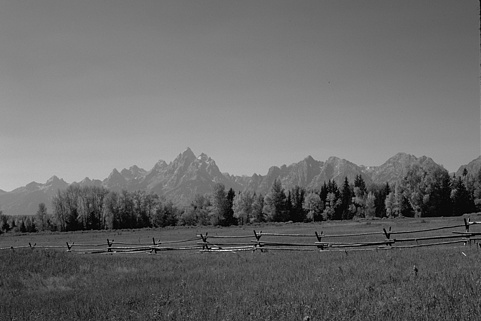
\includegraphics[width=10cm,height=7cm]{1}\begin{center}
	\small Fig.1 Simulation Result
\end{center}
Basically, their algorithm performs a task of matrix completion when there is incomplete data matrix. For matrix completion they use nuclear norm.By comparing two nuclear norm heuristics algorithm can know the location of the corrupted entry and using an augmented Lagrange multiplier algorithm they minimize the nuclear norm. $\lVert L-L_0 \rVert_F / \lVert L_0 \rVert_F \textless 10^{-3}$ 


\section{ALGORITHM}
In this article they choose solve the convex PCP problem (1.1) using an augmented Lagrange multiplier (ALM) algorithm. In their experience, ALM achieves much higher
accuracy than APG (Accelerated Proximal Gradient), in fewer iterations. APG is generalized form of projection used to solve convex optimization problem. It works stably across a wide range of problem settings with no tuning of parameters. Moreover, we observe an appealing (empirical) property: the rank of the iterates often remains bounded by rank($L_0$)
throughout the optimization, allowing them to be computed especially efficiently. APG, on the other hand, does not have this property.

\section{Conclusion}
	
	For the given large data matrix with corrupted or missing entries it is possible to recover original data matrix entirely using PCP (Principal component pursuits) technique. Now a days it is widely used technique in real life application to recover corrupted data.There are many other real life application like video surveillance, face recognition, recommendation system and many other.
% Now we need a bibliography:
\begin{thebibliography}{9}
	\bibitem{1}
	E. CANDES, X. LI and J. WRIGHT, 2011. [Online]. Available: http://statweb.stanford.edu/~candes/papers/RobustPCA.pdf. [Accessed: 02- Feb- 2017].
	\bibitem{2}
	"Augmented Lagrangian Methods | NEOS", Neos-guide.org, 2017. [Online]. Available: https://neos-guide.org/content/augmented-lagrangian-methods. [Accessed: 04- Feb- 2017].
	\bibitem{3}
	"Proximal gradient method", En.wikipedia.org, 2017. $[Online]$. Available: \url{https://en.wikipedia.org/wiki/Proximal_gradient_method}. $[Accessed: 09- Feb- 2017]$.
	\bibitem{4}
	D. Laptev, "dlaptev/RobustPCA", GitHub, 2014. $[Online]$. Available: \url{https://github.com/dlaptev/RobustPCA}. [Accessed: 05- Feb- 2017].
	\bibitem{5}
	O. Kuybeda, G. Frank, A. Bartesaghi, M. Borgnia, S. Subramaniam and G. Sapiro, "A collaborative framework for 3D alignment and classification of heterogeneous subvolumes in cryo-electron tomography"
	\bibitem{6}
	"Optimization Problem Types - Convex Optimization", solver. $[Online]$. Available: \url{http://www.solver.com/convex-optimization}. [Accessed: 04- Feb- 2017].
	\bibitem{7}
	B. Narayan, 2016. $[Online]$. Available: \url{https://www.quora.com/What-is-the-significance-of-the-nuclear-norm}. [Accessed: 06- Feb- 2017].
	\bibitem{8}
	W. H, "l0-Norm, l1-Norm, l2-Norm, … , l-infinity Norm", Rorasa's blog. $[Online]$. Available: \url{https://rorasa.wordpress.com/2012/05/13/l0-norm-l1-norm-l2-norm-l-infinity-norm/}. [Accessed: 08- Feb- 2017].
	\bibitem{9}
	"Why is minimizing the nuclear norm of a matrix a good surrogate for minimizing the rank?", Math.stackexchange.com, 2016. [Online]. Available: http://math.stackexchange.com/questions/164208/why-is-minimizing-the-nuclear-norm-of-a-matrix-a-good-surrogate-for-minimizing-t. [Accessed: 03- Feb- 2017].
	
\end{thebibliography}



% Your document ends here!
\end{document}